%----------------------------------------------------------------
%
%  File    :  thesis.tex
%
%  Authors :  Keith Andrews, IICM, TU Graz, Austria
%             Manuel Koschuch, FH Campus Wien, Austria
%			  Sebastian Ukleja, FH Campus Wien, Austria
% 
%  Created :  22 Feb 96
% 
%  Changed :  14 Oct 2020
%
%  For suggestions and remarks write to: sebastian.ukleja@fh-campuswien.ac.at
% 
%----------------------------------------------------------------

% --- Setup for the document ------------------------------------

%Class for a book like style:
\documentclass[11pt,a4paper,oneside]{scrbook}
%For a more paper like style use this class instead:
%\documentclass[11pt,a4paper,oneside]{thesis}

%input encoding for windows in utf-8 needed for Ä,Ö,Ü etc..:
\usepackage[utf8]{inputenc}
%input encoding for linux:
%\usepackage[latin1]{inputenc}
%input encoding for mac:
%\usepackage[applemac]{inputenc}

\usepackage[english]{babel}
% for german use this line instead:
%\usepackage[ngerman]{babel}

%needed for font encoding
\usepackage[T1]{fontenc}

% want Arial? uncomment next two lines...
%\usepackage{uarial}
%\renewcommand{\familydefault}{\sfdefault}

%some formatting packages
\usepackage[bf,sf]{subfigure}
\renewcommand{\subfigtopskip}{0mm}
\renewcommand{\subfigcapmargin}{0mm}

%For better font resolution in pdf files
\usepackage{lmodern}

\usepackage{url}

%\usepackage{latexsym}

\usepackage{geometry} % define pagesize in more detail


\usepackage{colortbl} % define colored backgrounds for tables

\usepackage{courier} %for listings
\usepackage{listings} % nicer code formatting
\lstset{basicstyle=\ttfamily,breaklines=true}

\usepackage{graphicx}
  \pdfcompresslevel=9
  \pdfpageheight=297mm
  \pdfpagewidth=210mm
  \usepackage[         % hyperref should be last package loaded
    pdftex, 		   % needed for pdf compiling, DO NOT compile with LaTeX
    bookmarks,
    bookmarksnumbered,
    linktocpage,
    pagebackref,
    pdfview={Fit},
    pdfstartview={Fit},
    pdfpagemode=UseOutlines,                 % open bookmarks in Acrobat
  ]{hyperref}
\DeclareGraphicsExtensions{.pdf,.jpg,.png}
\usepackage{bookmark}

\usepackage[title]{appendix}

%paper format
\geometry{a4paper,left=30mm,right=25mm, top=30mm, bottom=30mm}

% --- Settings for header and footer ---------------------------------
\usepackage{scrlayer-scrpage}
\clearscrheadfoot
\pagestyle{scrheadings}
\automark{chapter}

\usepackage{csquotes}

%Left header shows chapter and chapter name, will not display on first chapter page use \ihead*{\leftmark} to show on every page
\ihead{\leftmark} 	
%\ohead*{\rightmark}	%optional right header
\ifoot*{Guntram Björn Klaus}	%left footer shows student name
\ofoot*{\thepage}		%right footer shows pagination
%---------------------------------------------------------------------

%Start of your document beginning with title page
\begin{document}


% --- Main Title Page ------------------------------------------------
\begin{titlepage}
\frontmatter

\begin{picture}(50,50)
\put(-70,40){\hbox{
\includegraphics{images/logo.png}}}
\end{picture}

\vspace*{-5.8cm}

\begin{center}

\vspace{6.2cm}

\hspace*{-1.0cm} {\LARGE \textbf{Hardening Kubernetes Clusters\\}}
\vspace{0.2cm}
\hspace*{-1.0cm}Reducing Attack Surface in Kubernetes by means of Rootless Containers, Network Policies and Role Based Access Control\\

\vspace{2.0cm}

\hspace*{-1.0cm} { \textbf{Bachelor Thesis\\}}

\vspace{0.65cm}

\hspace*{-1.0cm} Submitted in partial fulfillment of the requirements for the degree of \\

\vspace{0.65cm}

\hspace*{-1.0cm} \textbf{Bachelor of Science in Engineering\\}

\vspace{0.65cm}

\hspace*{-1.0cm} to the University of Applied Sciences FH Campus Wien \\
\vspace{0.2cm}
\hspace*{-1.0cm} Bachelor Degree Program: Computer Science and Digital Communications \\

\vspace{1.6cm}

\hspace*{-1.0cm} \textbf{Author:} \\
\vspace{0.2cm}
\hspace*{-1.0cm} Guntram Björn Klaus \\

\vspace{0.7cm}

\hspace*{-1.0cm} \textbf{Student identification number:}\\
\vspace{0.2cm}
\hspace*{-1.0cm} c2110475170 \\

\vspace{0.7cm}

\hspace*{-1.0cm} \textbf{Supervisor:} \\
\vspace{0.2cm}
\hspace*{-1.0cm} BSc. MSc. Bernhard Taufner \\

\vspace{0.7cm}

% Reviewer if needed
%\hspace*{-1.0cm} \textbf{Reviewer: (optional)} \\
%\vspace{0.2cm}
%\hspace*{-1.0cm} Title first name surname \\


\vspace{1.0cm}

\hspace*{-1.0cm} \textbf{Date:} \\
\vspace{0.2cm}
\hspace*{-1.0cm} dd.mm.yyyy \\

\end{center}
\end{titlepage}

\newpage

\vspace*{16cm}
\setcounter{page}{1}

% --- Declaration of authorship ------------------------------------------
\hspace*{-0.7cm} \underline{Declaration of authorship:}\\\\
I declare that this Bachelor Thesis has been written by myself. I have not used any other than the listed sources, nor have I received any unauthorized help.\\\\
I hereby certify that I have not submitted this Bachelor Thesis in any form (to a reviewer for assessment) either in Austria or abroad.\\\\
Furthermore, I assure that the (printed and electronic) copies I have submitted are identical.
\\\\\\
Date: \hspace{6cm} Signature:\\

% --- English Abstract ----------------------------------------------------
\cleardoublepage
\chapter*{Abstract}
(E.g. ``This thesis investigates...'')

% --- German Abstract ----------------------------------------------------
\cleardoublepage
\chapter*{Kurzfassung}
(Z.B. ``Diese Arbeit untersucht...'')


% --- Abbrevations ----------------------------------------------------
\chapter*{List of Abbreviations}
\vspace{0.65cm}

\begin{table*}[htbp]
		\begin{tabular}{ll}
			DNS & Domain Name System \\
      CPU & Central Processing Unit \\
      RAM & Random Access Memory \\
      OS & Operating System \\
      API & Application Programmable Interface \\
      REST & Representational State Transfer \\
      CNI & Container Network Interface \\
      JWT & JSON Web Token \\
      PV & Persistent Volume \\
      PVC & Persistent Volume Claim \\
      UTS & Unix Time Sharing \\
      IPC & Inter Process Communication \\
      POSIX & Portable Operating System Interface \\
		\end{tabular}
\end{table*}

% --- Key terms ----------------------------------------------------
\newpage
\chapter*{Key Terms}
\vspace{0.65cm}

\begin{itemize}
	\setlength{\itemsep}{0pt}
	\item[] Container
	\item[] Kubernetes
	\item[] Cloud
	\item[] Security
\end{itemize}

% --- Table of contents autogenerated ------------------------------------
\newpage
\tableofcontents
\thispagestyle{empty}

% --- Begin of Thesis ----------------------------------------------------
\mainmatter
\chapter{Introduction}
\label{chap:intro}

\section{Enterprises and Cloud}

Over the last years, there has been a significant shift in the way enterprises around the world deploy, scale and maintain the 
lifecycle of their computing infrastructure and the software that runs on top of it. Applications used to be primarily constructed 
as one large software unit that bundled all features, business logic, user interfaces and data access components.
Increasing necessity for scalability, flexibility and maintainability made organizations transition from such monolithic architectures
to microservices, which are smaller, separated but loosely coupled software units implementing one component of the larger system at hand.
The release of the Docker container platform in 2013 had a significant impact on making transitions from monoliths to microservices feasible.  
Kubernetes has since emerged as the go-to choice for managing containerized applications at scale, particularly in cloud-native environments.
Its ability to automate tasks, scale applications, and support a wide range of use cases makes it a powerful tool for both 
large enterprises and small teams. However, Kubernetes is a large and complex system that consists of many components including additional plugins. 
To ensure an enterprise grade, production ready Kubernetes environment, there are vast amounts of configurations to make. As a single
platform that abstracts orchestration, networking, storage, monitoring, access control and more, Kubernetes becomes open to attack from many different
angles. The complexity, customizability and vastness highlight the amount of precision required to implement Kubernetes for production environments.  
\label{sec:Unterkapitel1}

\section{State Of The Art}

\section{Related Work}

\section{Objectives And Methodology}
\label{sec:Unterkapitel2}

This thesis aims to explore the landscape of security in Kubernetes


\chapter{Concepts}
\label{chap:back}


\section{Containervirtualization}
\label{sec:Unterkapitel21}

The high level definition of a container is that of a lightweight, standalone, and executable software package 
A container bundles the code itself, any required runtime environments, dependencies, settings as well as system 
tools and libraries into an isolated environment, which is instantiated on the underlying host machine.  
Such isolated environments are defined in tangible, portable formats called container images. 
The isolation of environments is mainly attributed to the namespace and Cgroup technology of the Linux kernel.


\subsection{Linux Kernel}
The kernel:
The operating system kernel is the core component of any operating system. It acts as a communication bridge between a user's 
applications and the underlying hardware. It is responsible for managing the fundamental functionality of the system, from 
scheduling processes to providing resources to applications. The kernel performs a number of crucial functions, including 
low-level networking, disk storage, and the control of processes and memory. The primary goals of the kernel include:

\begin{itemize}
  \item Establish the process that will run next on the CPU
  \item Keep track of the amount of memory being used of each process
  \item Act as mediator between processes and hardware
  \item Handle requests for execution from the processes through system calls
\end{itemize}


The kernel performs its tasks in its own, designated part of the system memory called "kernel space". In contrast, custom applications
such as web-browsers, texteditors and mail clients run in "user space". Kernel space and user space are kept apart. While the kernel has access to all of the memory, processes 
operating in the user space can only access a portion of it by calling the kernel interface. Through such system calls, 
a user-level program invokes services from the kernel. 

\subsubsection{Linux Control Groups}
Cgroups, short for control groups, are a Linux kernel feature that limits, accounts for, and isolates the resource usage 
(CPU, memory, disk I/O, etc.) of a collection of processes. These limits are enforced by the kernel. They ensure that processes do not
consume excessive resources and that other processes can access the resources they need. 
Cgroups support hierarchical grouping of processes, allowing for flexible resource management based on application requirements and user-defined policies. 
Cgroups are used by Docker and container platforms to isolate and manage resource pool of containers. In a Kubernetes environment, the option
to implement resource requests and limits of pods are enabled by Cgroups.

\subsubsection{Linux Namespaces}
Namespaces are Linux kernel mechanisms that provide a hierarchical partitioning of the system environment. The Linux manpage
defines namespaces as followed. 
\newline
\newline
\blockquote
{A namespace wraps a global system resource in an abstraction that
makes it appear to the processes within the namespace that they
have their own isolated instance of the global resource.}
\newline
\newline
Linux provides seven main types of namespaces:

\begin{itemize}
  \item PID namespace: Isolates process IDs
  \item Network namespace: Isolates Network devices, stacks, ports, etc.
  \item User namespaces: Isolates user and group IDs
  \item UTS namespace: Isolates hostname and domain name
  \item Mount namespaces: Isolates mount points
  \item IPC namespace: Isolates System V IPC objects and POSIX message queues
  \item Cgroup namespaces: Isolates Cgroup root directory
\end{itemize}

\subsection{Container Images and Runtimes}
Piecing together aforementioned concepts, companies like Docker and RedHat, and initiatives such as the Open Container Interface, build 
sophisticated products and standards around these kernel features. A container image is a snapshot of a filesystem that contains the application's code, 
runtime, and dependencies. It encapsulates the entire environment required to run the application.
A container runtime is a software platform that manages the creation, execution, and lifecycle of containers based on an image
specification. It provides the underlying infrastructure and mechanisms for running isolated container instances.
Popular container runtimes include Docker Engine, Podman, and CRI-O.
The relationship between images and runtimes is that images are the blueprints for containers, while runtimes are the 
engines that bring them to life. The runtime receives a container image, extracts the required components, mounts the image's 
filesystem, creates cgroups and namespaces to instantiate the container environment.


\section{Kubernetes}
\label{sec:Unterkapitel23}
Kubernetes is an open-source system for managing containerized workloads and services. It provides a portable, extensible, 
and scalable platform that automates the deployment, scaling, and management of applications.
\subsection{Components}
A Kubernetes cluster is separated into a control plane and data plane. The control plane groups the components responsible for 
the underlying system of Kubernetes itself. The data plane hosts the actual user containers. Machines that run control-plane services
are referred to as master-nodes, whereas machines that host user applications are referred to as worker-nodes. 
There are four core control-plane components which work together to manage the cluster and ensure that applications run smoothly.
These components run as containers themselves inside the reserved 'kube-system' namespace. 

\subsubsection{API Server}
The API server is the entrance to the Kubernetes cluster. It provides a REST API that allows users and applications to interact 
with the cluster and manage its resources. The API server is responsible for handling requests from clients, validating them, and 
enforcing access control policies. It allows you to query the state of the cluster, as well as the configuration of all resources and the 
status of all pods.

\subsubsection{ETCD}
Etcd is a distributed key-value store that is used to store the cluster's state. It is highly available and replicated across multiple nodes, 
ensuring that the cluster's state is always consistent. Etcd is used by all of the control plane components to store information about the cluster, 
such as the configuration of resources and the status of pods.

\subsubsection{Kube Scheduler}
The scheduler is responsible for assigning pods to nodes in the cluster. It takes into account the resources available on each node, as well as the 
resource requirements of each pod, to ensure that pods are placed on nodes where they can run successfully. The scheduler also tries to spread pods 
across multiple nodes to improve availability and resilience. 

\subsubsection{Controller Manager}
The controller manager is a process that runs on each node in the cluster. It is responsible for monitoring the state of the cluster and taking corrective 
action when necessary. The controller manager watches for events, such as the creation or deletion of pods, and takes action to ensure that the cluster 
remains in a healthy state. For example, the controller manager can restart pods that are unhealthy or create new pods to meet demand. 

\subsubsection{Kube DNS}
In addition, Kube-DNS provides DNS resolution for services and pods within the cluster. It creates DNS records for services, allowing pods to reach services by name 
rather than IP address. This simplifies the process of accessing services and makes it more consistent with traditional application development without 
the need to map IP addresses to service names. It also  acts as the authoritative DNS server for the cluster's default domain, which is 'cluster.local'.
This ensures that DNS queries for names within the cluster are resolved correctly and consistently across all pods in the cluster. For example, if a service
named 'frontend' inside the 'myapp' namespace exposes an application, it can be called from another application inside the cluster via the domain 
'frontend.myapp.svc.cluster.local' or just 'frontend.myapp'. 

\subsubsection{Kubelet}
The Kubelet is an agent process that runs on each node in a Kubernetes cluster. Its primary responsibility is to manage the lifecycle of Kubernetes pods, which are the 
fundamental unit of deployment in Kubernetes. Kubelet ensures that pods are running, healthy, and up-to-date with the desired state. It also interacts with the Container 
Runtime Interface (CRI) to run and manage containers, and it communicates with the Kubernetes API server to retrieve and update pod information.

\subsubsection{Kube Proxy}
Next to the Kubelet, the Kube-proxy, is a network proxy that runs on each node in a Kubernetes cluster. It is responsible for maintaining network connectivity between pods and 
services. Services are abstractions that represent groups of pods that expose their endpoints to the outside world. Kube-proxy translates service definitions into network 
rules that direct traffic to the appropriate pods. This ensures that requests to a service are routed to the correct pods, even if the pods are dynamically provisioned or scaled.
Figure 2.1 gives a high level overview over Kubernetes components and concepts. 
\newline
\begin{figure}[htbp]
  \centering
      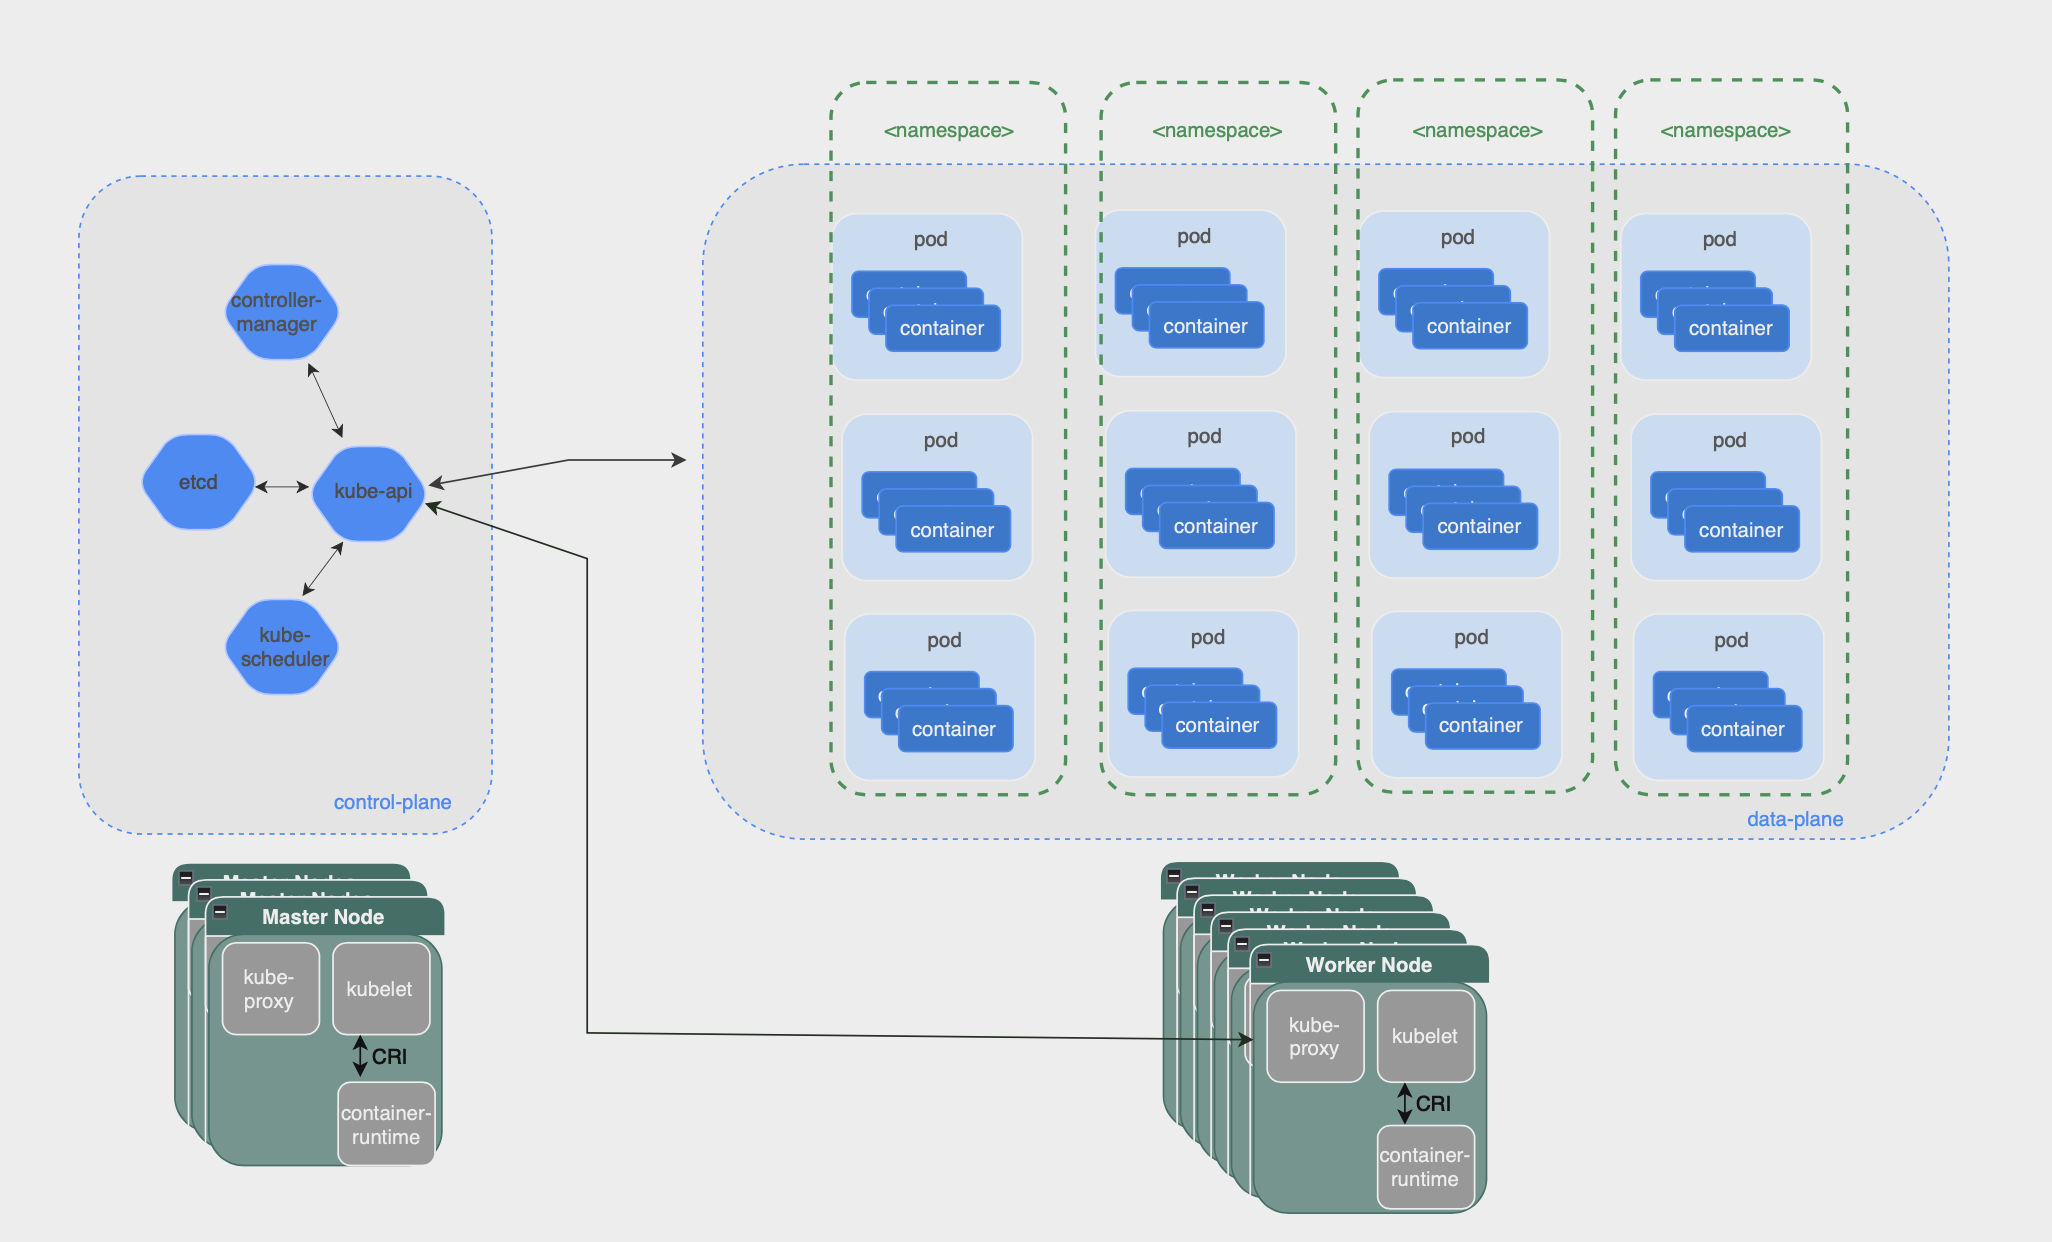
\includegraphics[height=10cm]{../images/kubernetes}
  \caption{Kubernetes Architecture Diagram [source: author]}
  \label{fig:k8arch}
\end{figure}

\subsection{Core Cluster Objects}

Kubernetes Objects are detailed specifications of the desired state of an application and the cluster as a whole. 
Objects are formulated in YAML syntax and are communicated to the Kubernetes API using the 'kubectl' command line 
utility.

\subsubsection{Kubernetes Namespaces}
Namespaces are virtual partitions in Kubernetes that arrange and segregate resource groupings inside a single cluster. 
Through namespaces the cluster is logically separated into more manageable, smaller sections. Kubernetes objects which define 
the state of an application, such as 'Deployment', 'Service' and 'ConfigMap' are namespaced. Objects which define the cluster as a 
whole or which pertain to all applications in all namespaces are not namespaced and exist globally. 
Namespace isolation prevents unintended interactions or interference between applications, 
maintaining the integrity of each deployment. Namespaces can be assigned different security policies, allowing for the enforcement 
of custom authorization rules and access control mechanisms. This helps protect resources and restrict unauthorized access between 
selected namespaces within the cluster. 

\subsubsection{Pod}
In Kubernetes, pods are fundamental building blocks for deploying and managing containerized applications. 
A pod is a group of one or more containers, which are tightly coupled and share resources such as network 
namespaces and filesystems. This tight coupling allows pods to be treated as a single unit for scheduling, 
management, and resource allocation. Pods expose the ports exposed by its containers, allowing external traffic 
to reach its intendend recipient. 

\subsubsection{Deployment}
Deployments describe the desired state of an application. A Deployment defines containers of pods, amount of pod replicas, 
hostnames, security settings, rolling update specifications and more. Its the central object for instantiating applications in Kubernetes.  

\subsubsection{Service}
In Kubernetes, a Service is an abstraction layer that defines a logical grouping of Pods and exposes them as a single, 
unified resource to the network. It simplifies the process of accessing and managing Pods by providing a stable endpoint 
and load balancing capabilities. Providing a stable endpoint ensures that pods can dynamically scale in the background 
with changing IP addresses. Services can be resolved to DNS names, providing a consistent and human-readable way to address the application.
Service objects use selectors to identify the Pods that belong to the Service.

\subsubsection{ConfigMap}
A ConfigMap is a key-value data store that can be mounted into Pods as environment variables, files, or command-line arguments. 
It provides a way to decouple configuration data from container images, making applications more portable and flexible.

\subsubsection{Ingress}
In Kubernetes, an Ingress is a controller that manages external traffic routing to a set of Services within the cluster. It acts as a 
front door for applications, handling load balancing, SSL termination, and other advanced traffic management tasks.
They direct external traffic to the appropriate services within the cluster. Ingresses support SSL/TLS termination, routing traffic based on the request's path, headers or query parameters, 
and more.

\subsubsection{ServiceAccount}
A ServiceAccount is a security identity that allows pods to access Kubernetes resources and services. It acts as an authentication mechanism for pods, managing their access 
permissions and controlling their interactions with the cluster. ServiceAccounts can mount Secrets into Pods, providing them with access to sensitive data such as passwords, 
API keys, or certificates.

\subsubsection{PersistentVolume and PersistentVolumeClaim}
In Kubernetes, a PersistentVolume is a storage resource that provides persistent storage to Pods. It ensures that data remains accessible even after Pods are terminated and 
recreated. A PersistentVolumeClaim object is a request for persistent storage from a Kubernetes pod. It defines the desired storage characteristics and specifications, such as storage capacity and access modes.
A PVC is referenced in a Deployment object. 

\subsubsection{NetworkPolicy}
A NetworkPolicy object defines rules for controlling network traffic between Pods. 
It allows for fine-grained control over network access, ensuring that Pods can only communicate with authorized sources and destinations.
The rules are enforced by the Kubernetes network plugin, ensuring that only authorized traffic is allowed to pass between pods.

\newpage
\chapter{Literature Review}

\section{Surveys}
It is evident that the reliance on Kubernetes comes with the need of a clear security initiative. According to RedHat's report on 
the state of Kubernetes security of 2022, more than ninety percent of polled organizations underwent at least one security incident
in their Kubernetes environment, which, in a third of cases, lead to the loss of revenue or customers. The majority of these incidents 
were detections of misconfigurations. About a third of respondents reported major vulnerabilities and runtime security incidents 
in relation to containers and/or Kubernetes which required immediate remediation. In a more recent, similar report conducted by RedHat in
2023, two thirds of respondents had to delay or slow down application deployments because of security concerns. This is a significant
increase compared to the 2022 survey, where just over half of participants experienced delays. Three of the most frequently mentioned 
advantages of containerization include quicker release cycles, quicker bug fixes, and increased flexibility to operate and manage applications. 
But if security is neglected, you can lose out on containerization's biggest benefit: agility.
It becomes apparent that Kubernetes is not something that is installed once and then never looked at again. Rather, a container-based 
environement that leverages this orchestration technology requires attention for detail and constant, rigurous inspection, despite the 
great amount of abstraction provided and due to its highly customizable nature.  CITE REDHAT 2022 2023

\section{CVE Scores}
Kubernetes is highly customizable and offers a range of configuration options which determine the security posture of
individual applications and the cluster as a whole. 
The purpose of this literature review is to explore the security threat landscape of Kubernetes environments. 
Specifically, recurring concepts and common denominators across vulnerabilities shall be identified and discussed. For this, 
the database of Common Vulnerabilities and Exposures (CVE), the IEEE database, the ACM digital library and the official
Kubernetes feed of CVEs are queried using keywords pertaining to Container and Kubernetes Security. In order to minimize manual 
labor to research the sheer amount of CVE reports, a Python script was developed to automate the research. The acquired papers, 
articles and CVE descriptions are skimmed through. The most relevant results are narrowed down and selected for closer inspection. 
It shall be noted that Kubernetes vulnerabilities do not only entail standard Kubernetes components, but also add-ons deployed on
top of 'plain' Kubernetes. Such can be the Nginx Ingress-Controller, a Service-Mesh, CI/CD tools closely embedded into Kubernetes
and more. Generally, this can be anything that extends the Kubernetes API through Custom Resource Definitions (CRDs).    
\\
CVE:
The main goal of the Common Vulnerabilities and Exposures (CVE) Programme is to identify vulnerabilities in a unique way and link particular 
code bases (such as common libraries and software) to those vulnerabilities. The usage of CVEs guarantees that when discussing or exchanging 
information about a specific vulnerability, two or more parties can confidently refer to a CVE identifier (CVE numbers). The CVE program 
defines a vulnerability as: 
\\
"A weakness in the computational logic (e.g., code) found in software and hardware components that, when exploited, results in a negative impact 
to confidentiality, integrity, or availability. Mitigation of the vulnerabilities in this context typically involves coding changes, but could 
also include specification changes or even specification deprecations (e.g., removal of affected protocols or functionality in their entirety)."
\\
In addition, the Common Vulnerability Scoring System (CVSS) "is a method used to supply a qualitative measure of severity"CITE HERE. 
The three metric groups that make up CVSS are Base, Temporal, and Environmental. Once the Temporal and Environmental metrics have been scored, 
the Base metrics produce a score between 0 and 10. A vector string, which is a condensed textual representation of the values required to calculate 
the score, is another way to visualise a CVSS score. Therefore, enterprises, organisations, and governments that require precise and consistent 
vulnerability severity scores can benefit greatly from using CVSS as a standard measurement system. CVSS is frequently used to prioritise vulnerability 
mitigation efforts and to determine the severity of vulnerabilities found on a system. All publicly available CVE records are assessed by the National
Vulnerability Database (NVD).
\\
There are multiple public APIs which allow for querying for various information on CVEs. The goal of the Python script is to quickly
collect CVEs for a given keyword with a CVSS base score higher than a given integer. To achieve this, the OpenCVE project's API is queried for all CVEs
containing a given keyword. The returned JSON response is filtered for the CVE number. This number is then used to call the NVD API of the NIST organization,
whose response can then be filtered for the base severity score according to the CVSS framework. As a result, interesting insights can be gained by
programmatic means. The following figure depicts the collected data on CVE's for the keyword 'Kubernetes'.
\\
\\
Total results: 269
\\
Base score average: 7.13
\\
Base score median: 7.2
\\
Base score modus: 6.5
\\
\\

\begin{figure}[htbp]
	  \centering
		    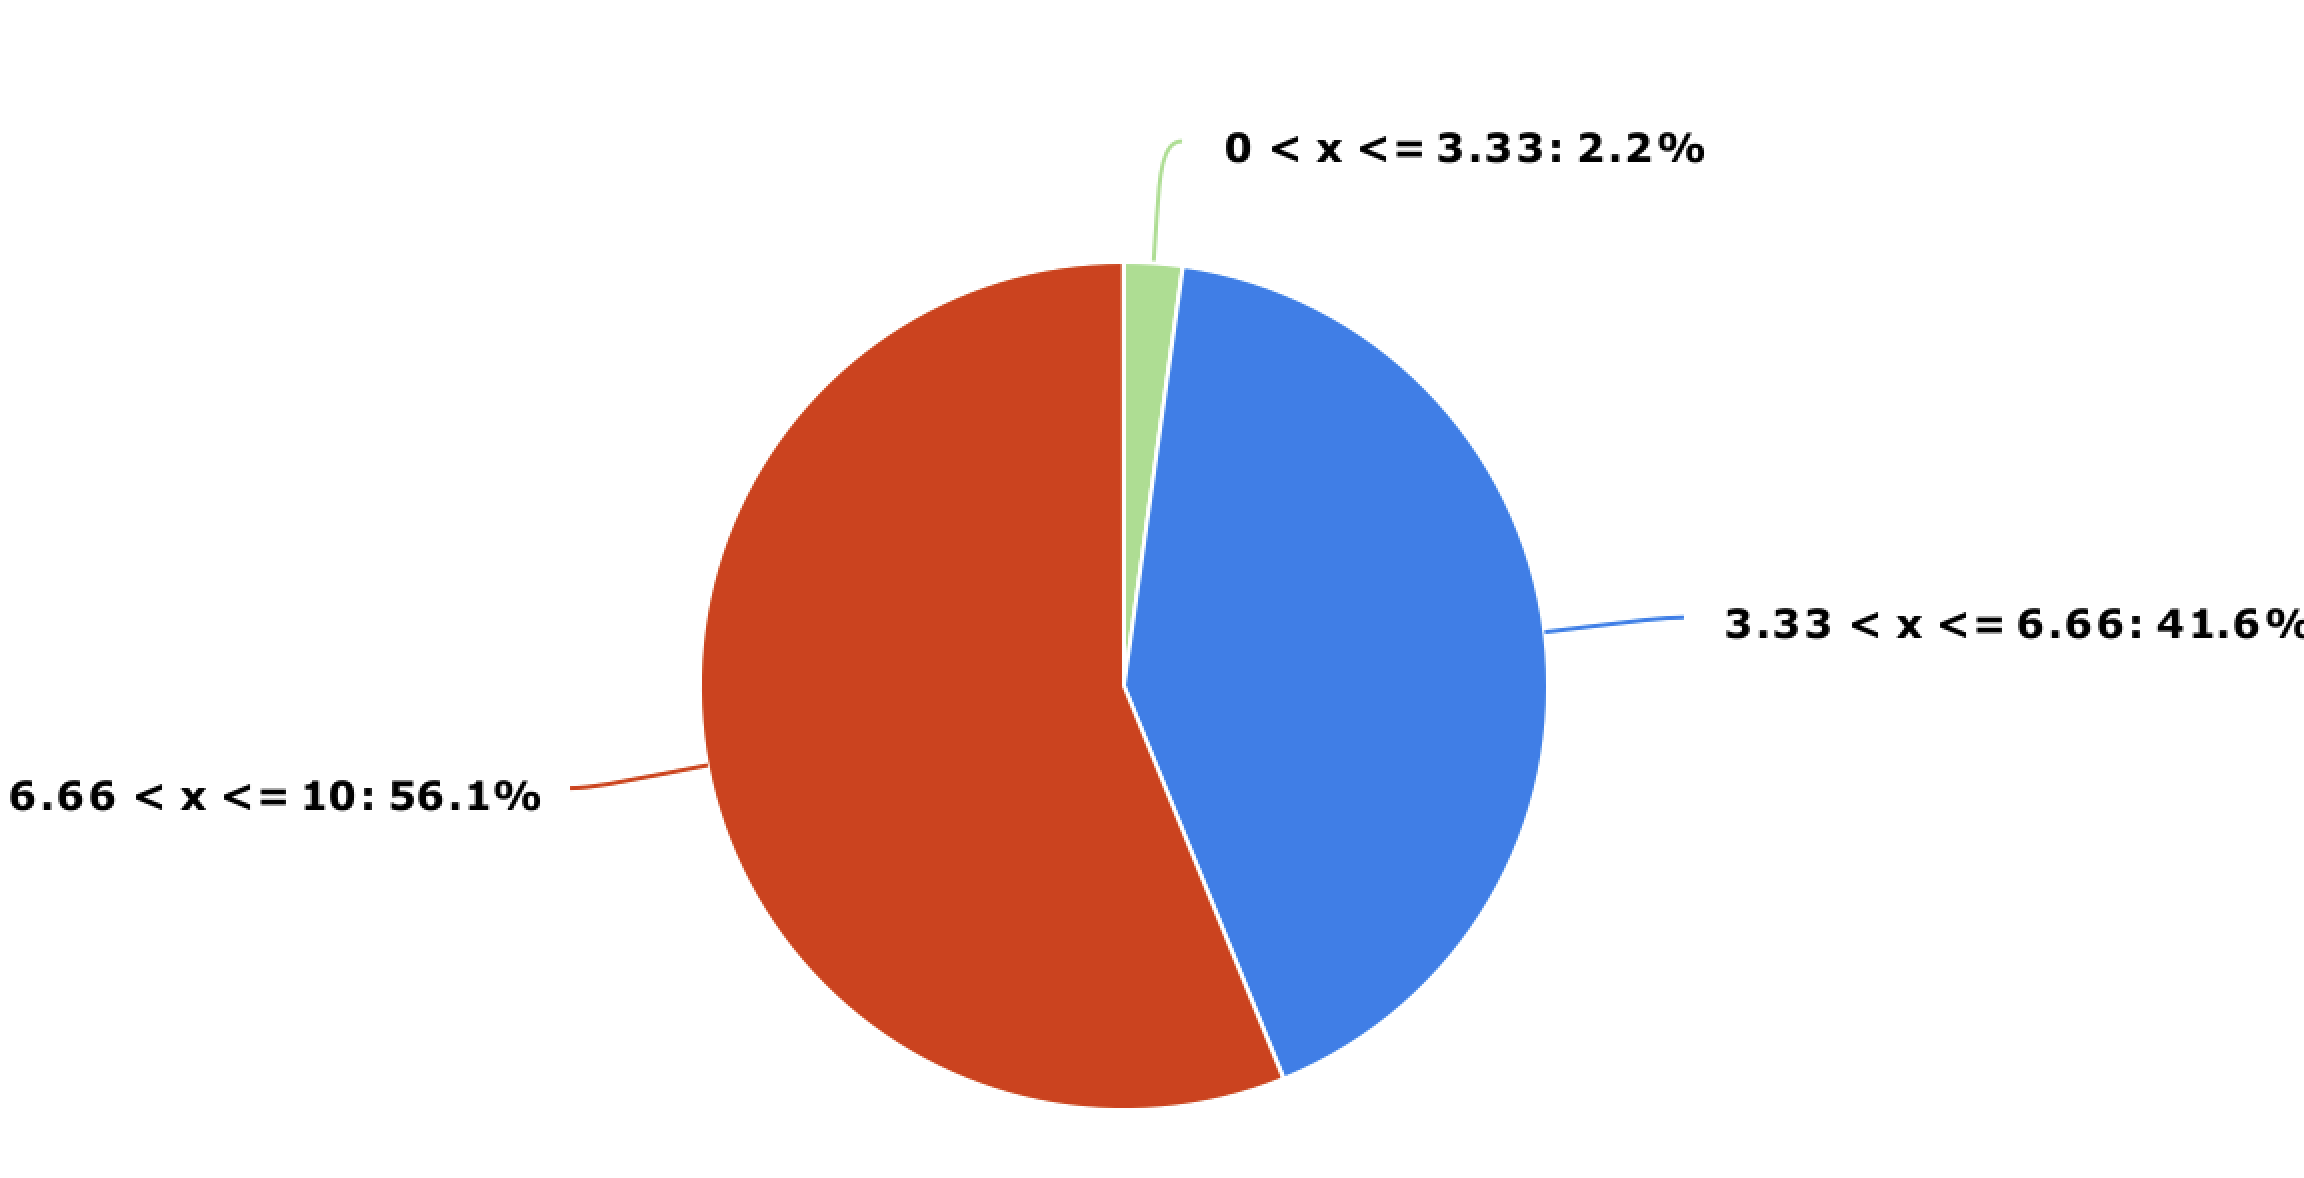
\includegraphics[height=5cm]{../images/cvepie}
	  \caption{Makeup of base scores of CVEs about Kubernetes}
	  \label{fig:cvepie}
\end{figure}


The chart below depicts the collected data on CVE's containing either of the keywords 'containerd', 'CRI-O' or 'Docker Container'.
\\
\\
Total results: 75
\\
Base score average: 7.9
\\
Base score median: 7.8
\\
Base score modus: 9.8
\\
\\
\begin{figure}[htbp]
  \centering
      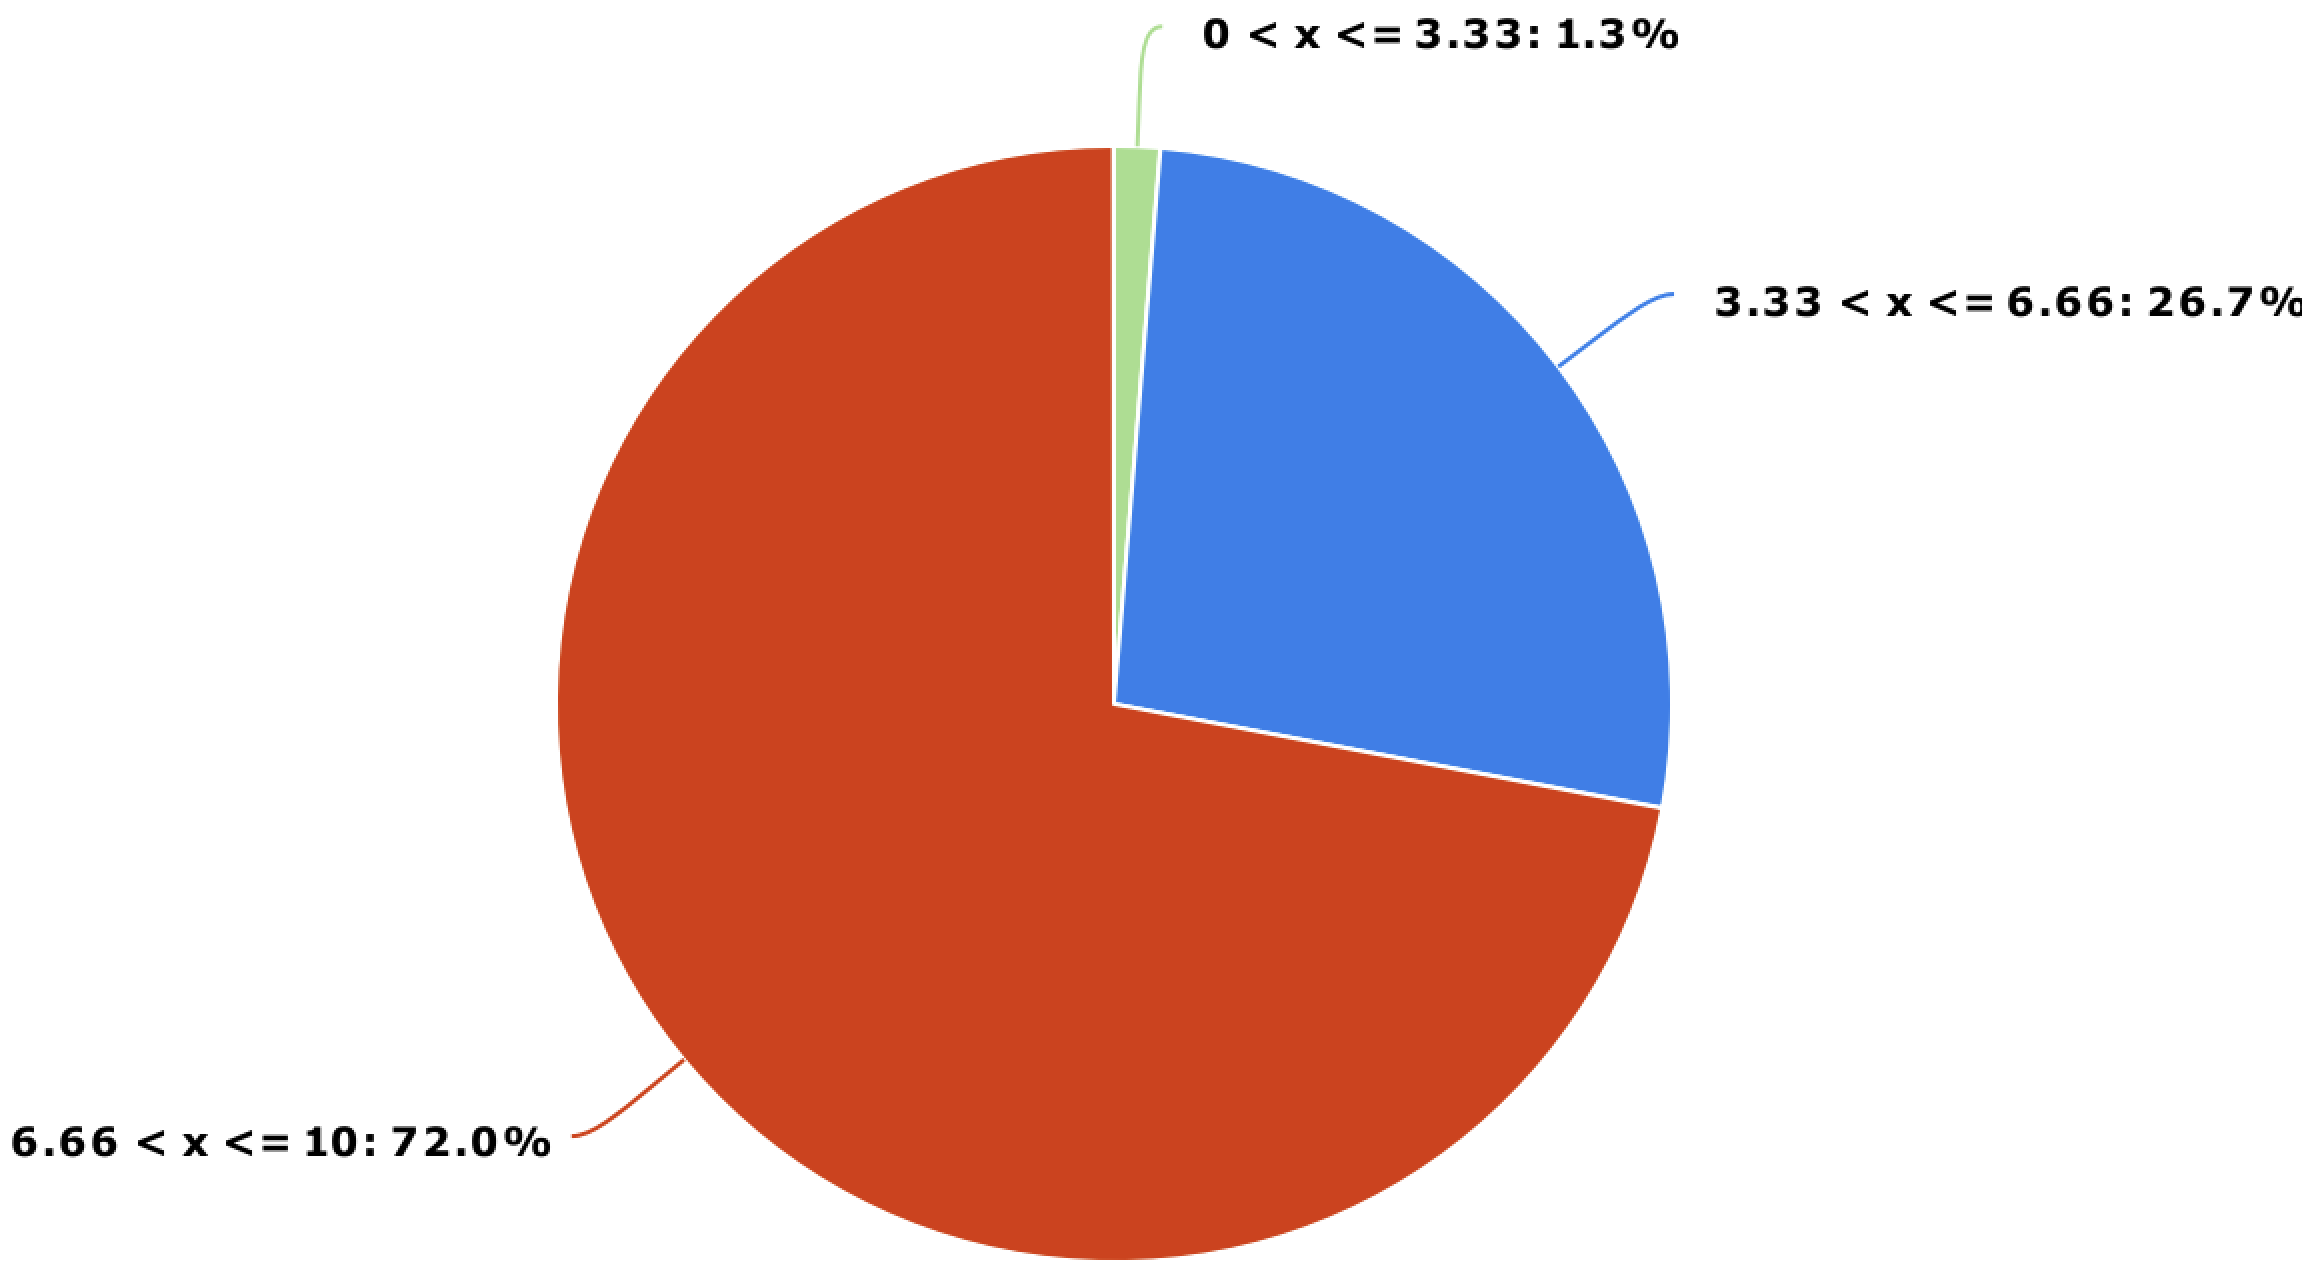
\includegraphics[height=5cm]{../images/cvepie2}
  \caption{Makeup of base scores of CVEs about Kubernetes}
  \label{fig:cvepie}
\end{figure}

Based on collected data, it is noticeable that CVSS base severity scores in the realm of Containervirtualization and Kubernetes tend toward extremes
on the higher end. For the keyword 'Kubernetes', more than half of CVEs are rated with a base score higher than 6.66, while there are hardly any 
scores smaller than 3.33. For CVEs that draw on popular container runtimes, an overwhelming majority close to 75 percent of cases holds base scores 
between 6.66 and 10. Here, once again, scores smaller than 3.33 are low. These two observations additionally emphasize the necessity for clear 
security measures when orchestrating containers in Kubernetes. 
The script enables to quickly retrieve the tendencially more severe vulnerabilities. Some CVEs marked with a CVSS base scores higher than 7 shall
be explored in the following chapters.

\section{CVE Reports}

\subsubsection {Container Escape}
Major vulnerabilities include those which fall under the category of a so called container-escape. Since a container is intended to be a 
runtime environment isolated from the underlying host, the concept of a container-escape relates to performing an exploit that breaks the confines 
of exactly this isolation, resulting in full or limited access to the underlying host machine and/or network. A study conducted by Reeves 
et al. at the end of 2021 investigates the susceptibility of different container runtime systems to escape-exploits by studying a batch of CVE 
reports. The study identifies three main causes for container escapes. 
First, mishandled file descriptors, if for example left accessible from within a container under /proc directory, provides malicious actors read and write 
access to the underlying host filesystem, as seen in CVE-2019-5736. In this reported vulnerability, a container is set up with a symlink from the 
container's entrypoint to proc/self/exe, which points back to its runC binary, which instantiated the container process. In addition, the container 
carries a harmful file which is designed to overwrite the  file descriptors of any excecuting process that loads it. If an unknowing person executes 
a binary within the container, which has been manipulated to symlink to /proc/self/exe, the harmful file is able to overwrite the runC binary. 
The next time another, unrelated container is spawned, it is done by the compromised runC binary. 
Secondly, missing access control to runtime components could enable adversaries to gain access to UNIX sockets on the host, as reported in 
CVE-2020-15257. Here, it was possible to connect to the containerd socket, thus enabling actors to issue API commands to freely create new containers
on the host, unconstrained by Apparmor, seccomp, or Linux capabilities. 
Thirdly, under 'adversary-controlled host execution' problems of similar fashion to mishandled file descriptors are mentioned. In this case however, 
vulnerability exposure starts with host binaries being executed in the container context, which makes it a target for manipulation. 
In CVE-2019-101(44–47), the shared library "libc.so.6" is altered in such a way that it mounts the host filesystem when loaded. The new shell loads 
"libc.so" when the administrator runs "rkt-enter", which is the /bin/bash command by default, to create a new shell in the container. This sets off malicious 
code embedded in "libc.so", which uses the mknod syscall to construct a block device of the host root filesystem inside the container. 
As a result, the adversary is able to read and write to the host filesystem. 
\\
CVE-2022-0811, which is barely discussed in papers due to its young nature, reports a sophisticated container escape possibility of the CRI-O container engine.
Generally, the interface of the Linux kernel accepts parameters which control its behavior. This interface is consumed by CRI-O to set kernel options for a pod. 
However, the parameter input string is not checked or sanitized, which allows for injecting additional, otherwise undesired parameters. Specifically in the
example of CVE-2022-0811, the "kernel.core\_pattern" kernel parameter is specified within the parameter of the safe "kernel.shm\_rmid\_forced" parameter, 
which controls the kernel's reaction to a core dump. If a core dump is done in a CRI-O container, the parameter states the execution of a malicious binary. 
This binary sits inside the container but is invoked on the host in the root context of the container from the perspective of the kernel.
\\
CVE-2022-23648 is another vulnerability related to container-escape, this time found in Containerd, a popular Kubernetes runtime. This vulnerability lies in 
Containerd's CRI plugin that handles OCI image specs containing "Volumes". An attacker can exploit this vulnerability by adding a Volume containing path traversal 
to the image. This allows them to copy arbitrary files from the host to a container mounted path. More specifically, The vulnerability resides in the 
"copyExistingContents" function in Containerd's code. This function copies the files from the attacker-controlled volume path to a temporary folder that is later 
mounted inside a container. An attacker can trick this function into copying arbitrary files from the host filesystem using path traversal.
This can lead to the disclosure of confidential information. The severity of this vulnerability is rated as high, with a CVSS base score of 7.5.
\\
CVE-2022-1708 is a vulnerability found in Cri-o, a lightweight container runtime for Kubernetes. This vulnerability is related to the allocation of resources 
without any limits or throttling, which can lead to uncontrolled resource consumption. The official CVE description states: "The ExecSync request runs commands 
in a container and logs the output of the command. This output is then read by CRI-O after command execution, and it is read in a manner where the entire file 
corresponding to the output of the command is read in." It is thus possible to exhaust memory or disk space of the node when CRI-O reads an extensive output 
of the command. The vulnerability is rated as high, with a CVSS base score of 7.5 and targets system availability.
\\
Cilium is an eBPF-based solution for network connectivity between workloads in Kubernetes CLusters. CVE-2022-29179 reports yet another subjection to the risk of 
container breakouts.  The CVE number is not directly about a technique to gain access outside the container, it rather addresses a vulnerability in Cilium given a 
successful container escape. It explicitly mentions root containers as a prerequesite. According to this CVE entry, Cilium's service account in versions prior to
version 1.9.16 allowed for escalating privileges to those of a cluster admin. This gave adversaries the ability to delete cluster resources such as Pods and Nodes. 
The entry is marked with a base score of 8.2 which is considered high.
\\
CVE-2020-8554:
In the case of CVE-2020-8554, the source is a design defect in the External IPs and Load Balancer IPs components of Kubernetes Services. An application running on a collection 
of pods can be exposed as a network service in an abstract manner using Kubernetes Services. One or more IPs are used to access a service. When the cluster's nodes 
are deployed, traffic intended for the service IPs will be routed through one of the backing pods that comprise the service. By assigning IP addresses that are already 
being used by other endpoints (internal or external), a malevolent user might intercept all cluster traffic directed towards those IP addresses. 
With the service shown below, it used to be possible to intercept UDP traffic to IP 8.8.8.8, which is Google's DNS server, and direct it to the "evil-dns-server" 
pod when it is deployed to the cluster.

\begin{figure}[htbp]
  \centering
      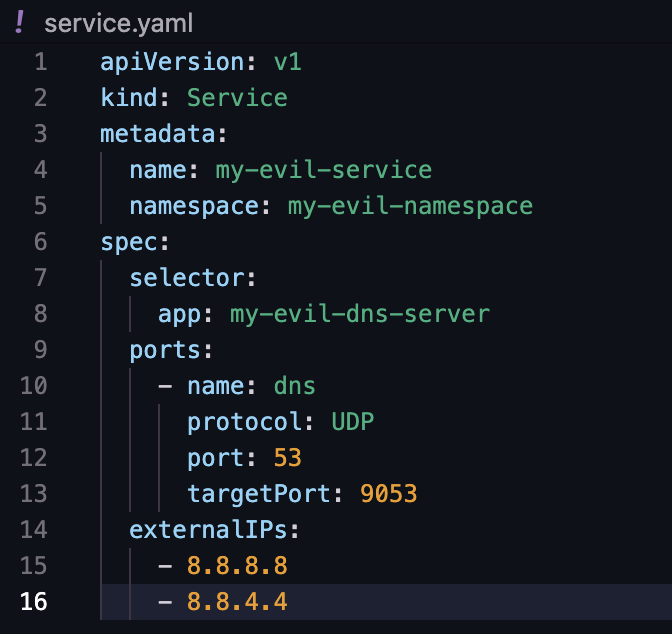
\includegraphics[height=5cm]{../images/service}
  \caption{YAML declaration of a malicious service}
  \label{fig:cvepie}
\end{figure}

Of the more recent vulnerabilities with high severity, CVE-2023-5043 and CVE-2023-5044 report problems with the Nginx Ingress Controller. 
The Nginx Ingress Controller is a popular add-on to Kubernetes with which cluster incoming traffic is managed. Instead of assigning
each Kubernetes Service an IP and port directly on the underlying node, the Nginx container serves as a single point of entry and acts as a reverse proxy to the cluster
workloads. To expose a cluster workload, a Kubernetes resource of type 'Ingress' is defined. Within this YAML definition, the nginx ingress controller picks up custom configuration
through so called annotation snippets. This allows for fine-grained, customized behavior of the controller for a respective service. It was however discovered that 
specific declarations of the "nginx.ingress.kubernetes.io/configuration-snippet" and "nginx.ingress.kubernetes.io/permanent-redirect" annotations of an Ingress Object can be 
used to inject arbitrary commands, making it possible to obtain credentials of the said nginx ingress controller. Utilizing this credential, even more cluster secrets could 
be obtained. Multi-tenant environments are most affected by the issue.  
\\
\\
As reported in  CVE-2022-24817, Flux2 can reconcile the state of a remote cluster when provided with a kubeconfig with the correct access rights. Kubeconfig files can define commands to be executed to generate 
on-demand authentication tokens. A malicious user with write access to a Flux source or direct access to the target cluster, could craft a kubeconfig to execute arbitrary code 
inside the controller’s container. In multi-tenancy deployments this can also lead to privilege escalation if the controller's service account has elevated permissions.
Within the affected versions range, one of the permissions set below would be required for the vulnerability to be exploited:
Direct access to the cluster to create Flux Kustomization or HelmRelease objects and Kubernetes Secrets.
Direct access to the cluster to modify existing Kubernetes secrets being used as kubeconfig in existing Flux Kustomization or HelmRelease objects.
Direct access to the cluster to modify existing Flux Kustomization or HelmRelease objects and access to create or modify existing Kubernetes secrets.
Access rights to make changes to a configured Flux Source. The vulnerability is marked with a CVSS base score of 9.9. 
\\
A successful container-escape arguably poses one of the greatest risk in a Kubernetes environment as it provides a starting point from which all three pillars of 
the CIA triad can be targeted: Confidentiality, Integrity, and Availability. Once an attacker gains access of the host, secrets can be read, binaries can be altered,
network traffic can be inspected and resources can be deleted. In contrast, other vulnerabilities 'only' allow for more restricted exploitability. For example, 
CVE-2022-1708, CVE------- and CVE---------- target the availability of the system, but not the confidentiality or integrity of data. The average CVE scores of
\\
The foundation of such attacks is being able to either freely instantiate containers or freely move and operate from inside a container
The most notable ones, which have a severity score above 8, according to the Common Vulnerability 
\\
We see that vulnerabilities vary tremendously in their appearance. CVE so and so targets a tool, CVE so and so targets the actual underlying
kernel of a k8s node. However, all these things can be prevented or alleviated by applying the concept of least privilege to containers, 
access to Kubernetes and the Kubernetes network. For example, if a malicious actor cannot freely create files in any desired directory of a 
compromised container, it significantly reduces his ability to exploit a given vulnerability. Not being able to create that file in the first 
place, due to missing write permissions, would be a major obstacle for performing a container escape. It is not always possible to completely 
avoid a vulnerability. This is due to software bugs and unidentified weaknesses in the code that have passed through the testing and review process. 


\chapter{Hardening Measures}
These are not problems exclusive to Kubernetes, they exist in any architecture using any tools, setups, services 
Measures are not exclusive to Kubernetes - containers 
Generally - regardless of the setup, tools and architecture used, granular access controls, network segmentation
or  
Kubernetes offers an insane range of configuration possibilitites out of the box / native kubernetes
or by installing custom tools inside the cluster. 

Principle of least privilege 



\section{Rootless Containers}

A rootless container is a container which runs its processes without root privileges. The root user in Linux is the account 
with the highest access rights on the instance. It can modify any system configuration, install and remove software packages, upgrade 
the operating system and firmware, read, write and execute any files on the system, and operate as any other user on the host. 
Any process that does not require such powerful access must be restricted in its permissions. The user which executes the application 
process inside the container must have the limited ability to perform only absolutely necessary actions to fulfill its purpose. 

\subsubsection{Dockerfile}

Running rootless containers in Kubernetes starts at the definition of the image. A Dockerfile is a text document which specifies 
commands to be executed for constructing the environment. This file is consumed by the Docker to build the image. The following 
Dockerfile, based on Alpine-Linux, installs nodejs, creates an unprivileged user with UID 1000, and assigns that user ownership
to the /app directory, from where it can run its application process. 

\begin{figure}[htbp]
  \centering
      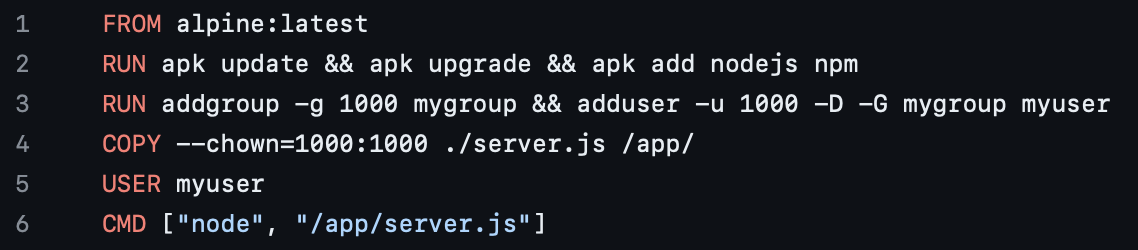
\includegraphics[width=10cm]{../images/dockerfile}
  \caption{Rootless image specification using Dockerfile}
  \label{fig:dockerfile}
\end{figure}


Kubernetes offers the 'securityContext' configuration section for declaration of pods, deployments and statefulsets.
Under 'securityContext', properties such as 'runAsNonRoot', 'runAsUser', 'allowPrivilegeEscalation' and 'readOnlyRootFilesystem' 
allow for restrictive access control settings inside containers. 

\subsubsection{runAsNonRoot}
The container is started with a non-root user ID (UID) rather than the normal root UID of 0 when runAsNonRoot is set to true. 
Whenever possible, it is advised to run containers as non-root to lower the risk of privilege escalation attacks. 
\subsubsection{runAsUser}
This setting in Kubernetes is used to specify the user ID that should be used to run the container. 
\subsubsection{allowPrivilegeEscalation}
This setting determines whether a container's privileges can be escalated. When true, it grants a container additional privileges 
beyond those granted by default. When set to false, obtaining higher privileges, by 'sudo' or 'setuid' operations for example, 
will be denied. 
\subsubsection{readOnlyRootFilesystem}
When set to true, this property ensures that the root filesystem is not writable.  
\newline
\newline
Linux offers different security architectures such as AppArmor, SELinux, and Seccomp. 
\subsubsection{Capabilities}
Capabilities are kernel level permissions that provide more precise control over kernel call permissions. Some examples of 
capabilities are the capacity to manage the network subsystem, modify file permissions, and carry out system-wide administrative 
tasks. Kubernetes offers configuration to remove or add capabilities using securityContext. Capabilities can be passed individually 
or as a comma-separated list in a string array. The -all shorthand is used to collectively drop or add all capabilitites. 
When the container runtime constructs the container, it uses this configuration to set capabilities. The container is 
given the default set of capabilities that the container runtime provides if the capabilities section is absent from 
the securityContext.
\subsubsection{AppArmor}
AppArmor is a Linux kernel security module that allows administrators to restrict programs' capabilities with per-program 
profiles. Profiles can allow capabilities like network access, raw socket access, and the permission to read, write, or execute files 
on matching paths. AppArmor is supported in Kubernetes through the securityContext field. 

\subsubsection{SELinux}
Security-Enhanced Linux (SELinux) is a security module for Linux systems that provides a mechanism for supporting fine-grained
access control security policies. Theconfiguration component of SELinux is a so called context label which defines permissions 
through combinations of user roles, types, levels, and security classes.  
The securityContext allows administrators to define such labels for Kubernetes deployments.  
The SELinux security module must be loaded on the host operating system to assing SELinux labels. 

\subsubsection{Seccomp}
The Linux kernel's seccomp feature can be used to restrict allowed system calls of a process, 
thereby lowering the kernel's attack surface. The set of system calls that the container is permitted to make is specified by 
seccomp-profiles also defined under securityContext. 
\newline
\newline
Thus, compromising the container instance through a reverse shell, for example, gives perpatrators limited ability to operate 
from inside the container, or break out of the container instance. 



\section{Network} 

A fresh installation of Kubernetes has no restrictions on network communication. Pods are free to receive ingress traffic from and send egress
traffic to any other endpoints inside the cluster or the outside world. This overly permissive default setting must be restricted by applying 
'NetworkPolicy' objects. Such objects require the installation of a Container Networking Interface (CNI) on top of Kubernetes. CNIs are Kubernetes
plugins which set up the network environment of the cluster. It handles network interfaces, IP addresses and routing of traffic of containers.  A CNI is a prerequesite 
for implementing Ingress, Service and NetworkPolicy objects. The NetworkPolicy rules work at Layer 3 (Network) and Layer 4 (Transport) of the OSI model. 
The following figure depicts a NetworkPolicy object which blocks all ingress and egress traffic. 

\begin{figure}[htbp]
  \centering
      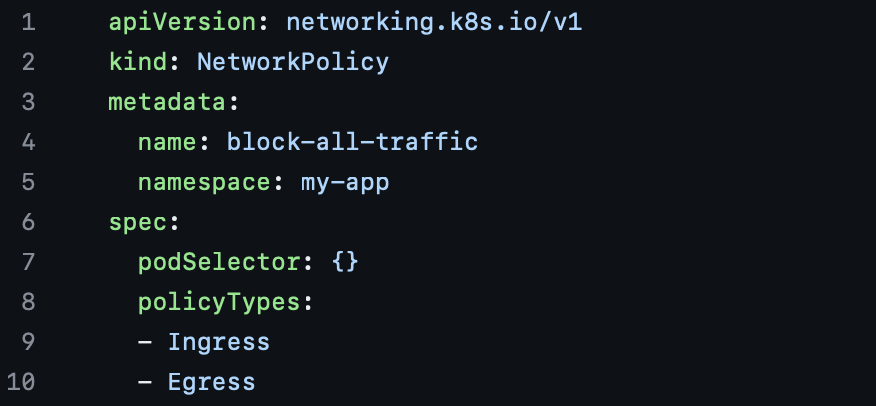
\includegraphics[height=3.5cm]{../images/nwp}
  \caption{A NetworkPolicy blocking all ingress and egress [source: author]}
  \label{fig:cvepie}
\end{figure}
NetworkPolicies are additive. If there is a policy allowing traffic for certain IPs, ports and namespaces, it overrules a blocking policy. 
The following figure depicts a NetworkPolicy object which whitelists incoming traffic from the app-x namespace and outgoing traffic to the 
public IP of 91.213.77.62 on port 443. \newline

\begin{figure}[htbp]
  \centering
      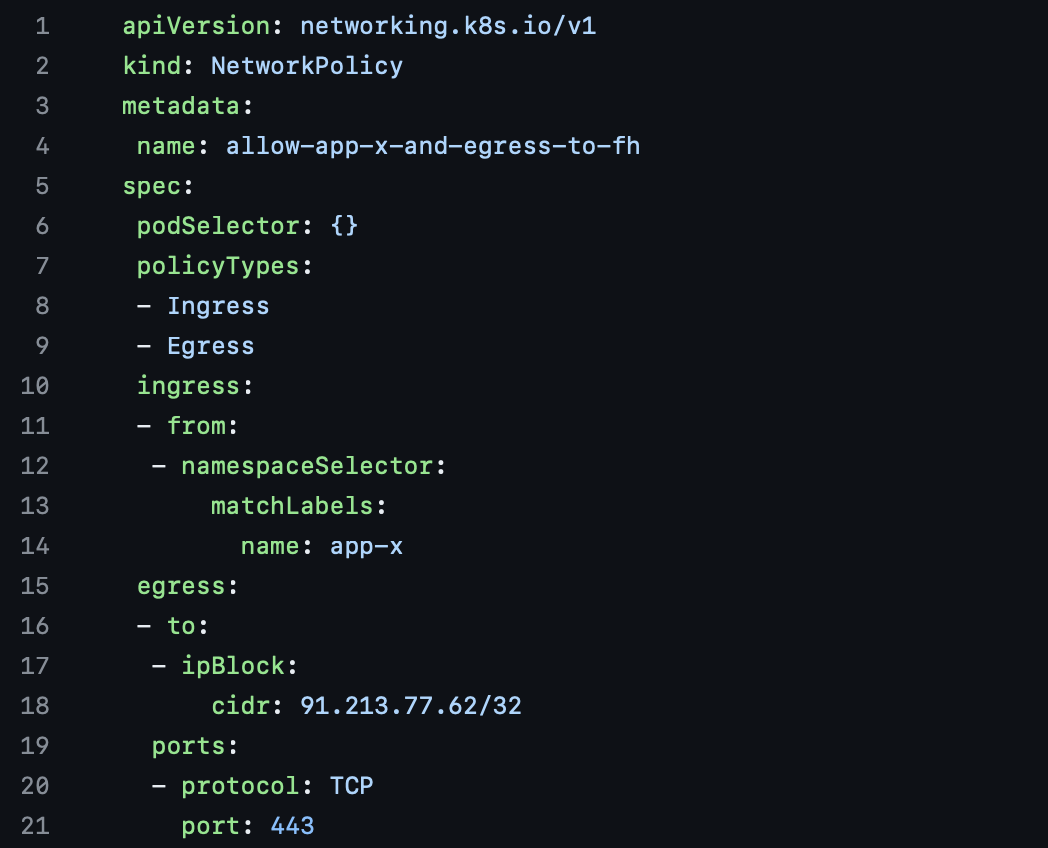
\includegraphics[height=6.5cm]{../images/nwp2}
  \caption{A NetworkPolicy allowing ingress from a namespace and egress to a public IP [source: author]}
  \label{fig:cvepie}
\end{figure}
\newpage
Standard NetworkPolicies are simple yet effective means to allow only the absolutely necessary origins and destinations of pod connections.
More fine grained and powerful settings can be achieved through the implementation of a service-mesh. Istio and Linkerd, popular service-mesh solutions
enable mutual TLS authentication in Kubernetes clusters. mTLS, an extension of standard TLS, requires both
parties to authenticate themselves, instead of just the server authenticating itself to the client. In mTLS, both client and server 
present and verify certificates to establish a secure connection. mTLS is a crucial component for implementing zero trust networks.
In addition to mTLS, service mesh solutions such as Linkerd and Istio provide AuthorizationPolicy objects. AuthorizationPolicies are used
to granularly control access to specific endpoints of specific services with specific authorization protocols within the cluster.   
Figure 4.4 is an example of an Istio AuthorizationPolicy object, which implements the following rules for all pods inside the 'foo' namespace:

\begin{itemize}
  \item Requests by pods identifying themselves with the cluster.local/ns/default/sa/sleep service account are allowed
  \item Request by pods inside the 'test' namespace are allowed
  \item GET methods to /info are only allowed when requests carry valid JWT issued by accounts.google.com
  \item POST methods to /data are only allowed when requests carry valid JWT issued by accounts.google.com
  \item Any other requests are denied 
\end{itemize}

\begin{figure}[htbp]
  \centering
      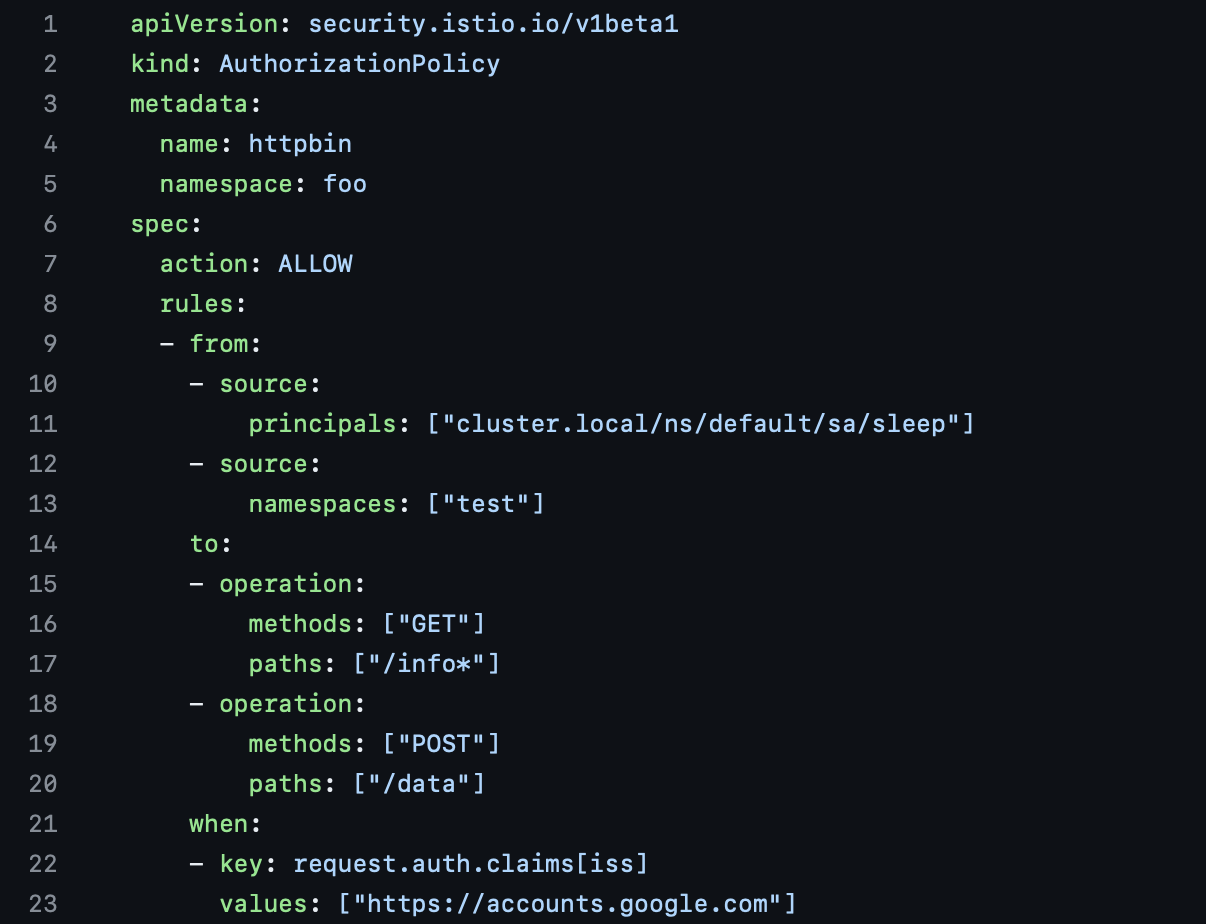
\includegraphics[height=6.5cm]{../images/authpolicy}
  \caption{Granular access control with AuthorizationPolicy [source: Istio ]}
  \label{fig:cvepie}
\end{figure}



\newpage
\section{Role Based Access Control}

Roles - bindings 
ClusterRoles - bindings
ServiceAccounts 

\chapter{Discussion}
\section{Implications for businesses}
\newpage
\section{Tradeoffs and Difficulties}
\section{Complexity}

\newpage
\chapter{Conclusion}

\newpage
\chapter{Outlook / Future work}

\newpage

% --- Bibliography ------------------------------------------------------

%IEEE Citation [1]
\bibliographystyle{IEEEtran}
%for alphanumeric citation eg.: [ABC19]
%\bibliographystyle{alpha}

% List references I definitely want in the bibliography,
% regardless of whether or not I cite them in the thesis.

\newpage
\addcontentsline{toc}{chapter}{Bibliography}
\bibliography{testBib}

\newpage

% --- List of Figures ----------------------------------------------------

\addcontentsline{toc}{chapter}{List of Figures}
\listoffigures


% --- List of Tables -----------------------------------------------------

\newpage
\addcontentsline{toc}{chapter}{List of Tables}
\listoftables

% --- Appendix A -----------------------------------------------------

\backmatter
\appendix
\begin{appendices}
\chapter{Appendix}

cve.py
\clearpage
\end{appendices}

\end{document}
